\chapter{Modernising Rate Monitoring Tools}
\label{ratemon}

One of the major challenges for the Compact Muon Solenoid (CMS) experiment, is the task of reducing event rate from roughly 40 MHz down to a more manageable 1 kHz while keeping as many interesting physics events as possible. This is accomplished through the use of a Level-1 (L1) hardware based trigger as well as a software based High-Level Trigger (HLT). Monitoring and understanding the output rates of the L1 and HLT triggers is of key importance for determining the overall performance of the trigger system and is intimately tied to what type of data is being recorded for physics analyses.

Here, we introduce the Trigger System in operation at the CMS experiment and proceed giving an overview of the software development work done to improve and add new features to the CMS Rate Monitoring software, a collection of tools used by CMS shifters to monitor the L1 and HLT trigger rates. Some additional experimental components have ben developed to showcase possible upgrades, delivering quality of life enhancements and enabling shifters and physicists to navigate data in a faster and more comfortable way.

Finally, proper export functionalities have been added to the tools, allowing to save and export Trigger Rates as JSON or ROOT binary files.

This work is also described in \cite{VivaceRTM1} \cite{VivaceRTM2} \cite{L1TriggerOMSDevelopments} \cite{MohrmanRTM}, the source code is available in the RateMon git repository \cite{RateMonGit}.

\section{CMS Trigger System}

A Trigger is an  electronic system for spotting potentially interesting collisions in a particle detector and triggering the detector’s read-out system to record the data resulting from the collision.

\begin{figure}
    \centerline{
        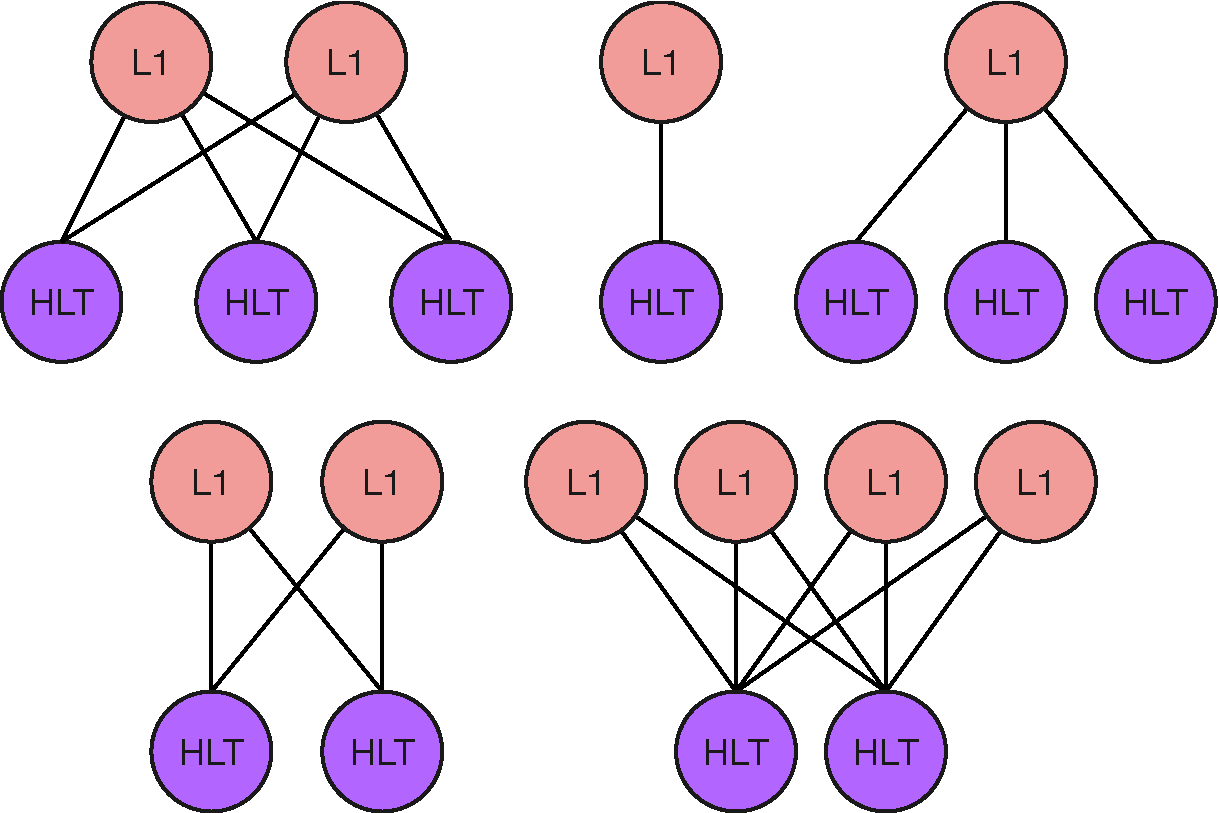
\includegraphics[width=0.5\paperwidth]{figures/triggers.pdf}}
    \caption{Simplified graph inspired by the trigger system configuration: the triggers connections can be seen as hierarchical directional graph. Red nodes represent L1 Trigger while purple HLT. Each link is directed from the red nodes to the purple ones. In reality, few hundred nodes spread approximately equally between HLT and L1 Trigger. \cite{adpol-cvae}}
    \label{fig:triggers}
\end{figure}


The LHC generates 40 millions events per second. Each event recorded by the CMS detector, carries on average a payload of 1 MB of unprocessed informations. It is technologically impossible to retain this amount of data, due to hardware, software, network and storage constraints. Furthermore, most events represent uninteresting information for the current state of physics knowledge.

The \textit{CMS Trigger System} is designed to reduce the output stream to 1000 events per second, while preserving the physics reach of the experiment.
It is composed by a hierarchical set of rules, called Trigger Nodes (or Paths): each one probes a specific patterns (physics signature) in the event or looks for specific physics objects.

This happens in two steps:

\begin{enumerate}

    \item The first level (L1) \cite{Bayatyan:706847} brings the 40 MHz to a 100 kHz rate. Here, 350-400 \cite{Sirunyan:2721198} Trigger Algorithms (or "seeds") are implemented on custom electronics (FPGAs and ASICs) exploiting informations from sub-detector components.

    \item A configurable set of L1 Trigger Nodes seeds Triggers in the second level (HLT), implemented in software. The event stream is further refined, selecting an average rate of 400 Hz for offline event storage and certification \cite{Khachatryan_2017}. HLT runs 400-500 of these independent Trigger Paths.

\end{enumerate}


\begin{table}
\begin{center}
 \begin{tabular}{||c c||} 
 \hline
 Algorithm & Requirements (GeV)\\ [0.5ex] 
 \hline\hline
 Single jet & $p_T > 180$ \\ 
 \hline
 Single tau lepton ($\mu$)      & $p_T > 22$ \& Tight Quality \\ 
  \hline
 Single electron/photon (e/$\gamma$) & $p_T > 36$ \& $|\eta| < 2.5$ \\ [1ex] 
 \hline
\end{tabular}
\caption{Some examples of unprescaled Level-1 trigger algorithms (seeds) used during Run 2 and their requirements \cite{Sirunyan:2721198}}
\end{center}
\end{table}


\begin{figure}
    \centerline{
        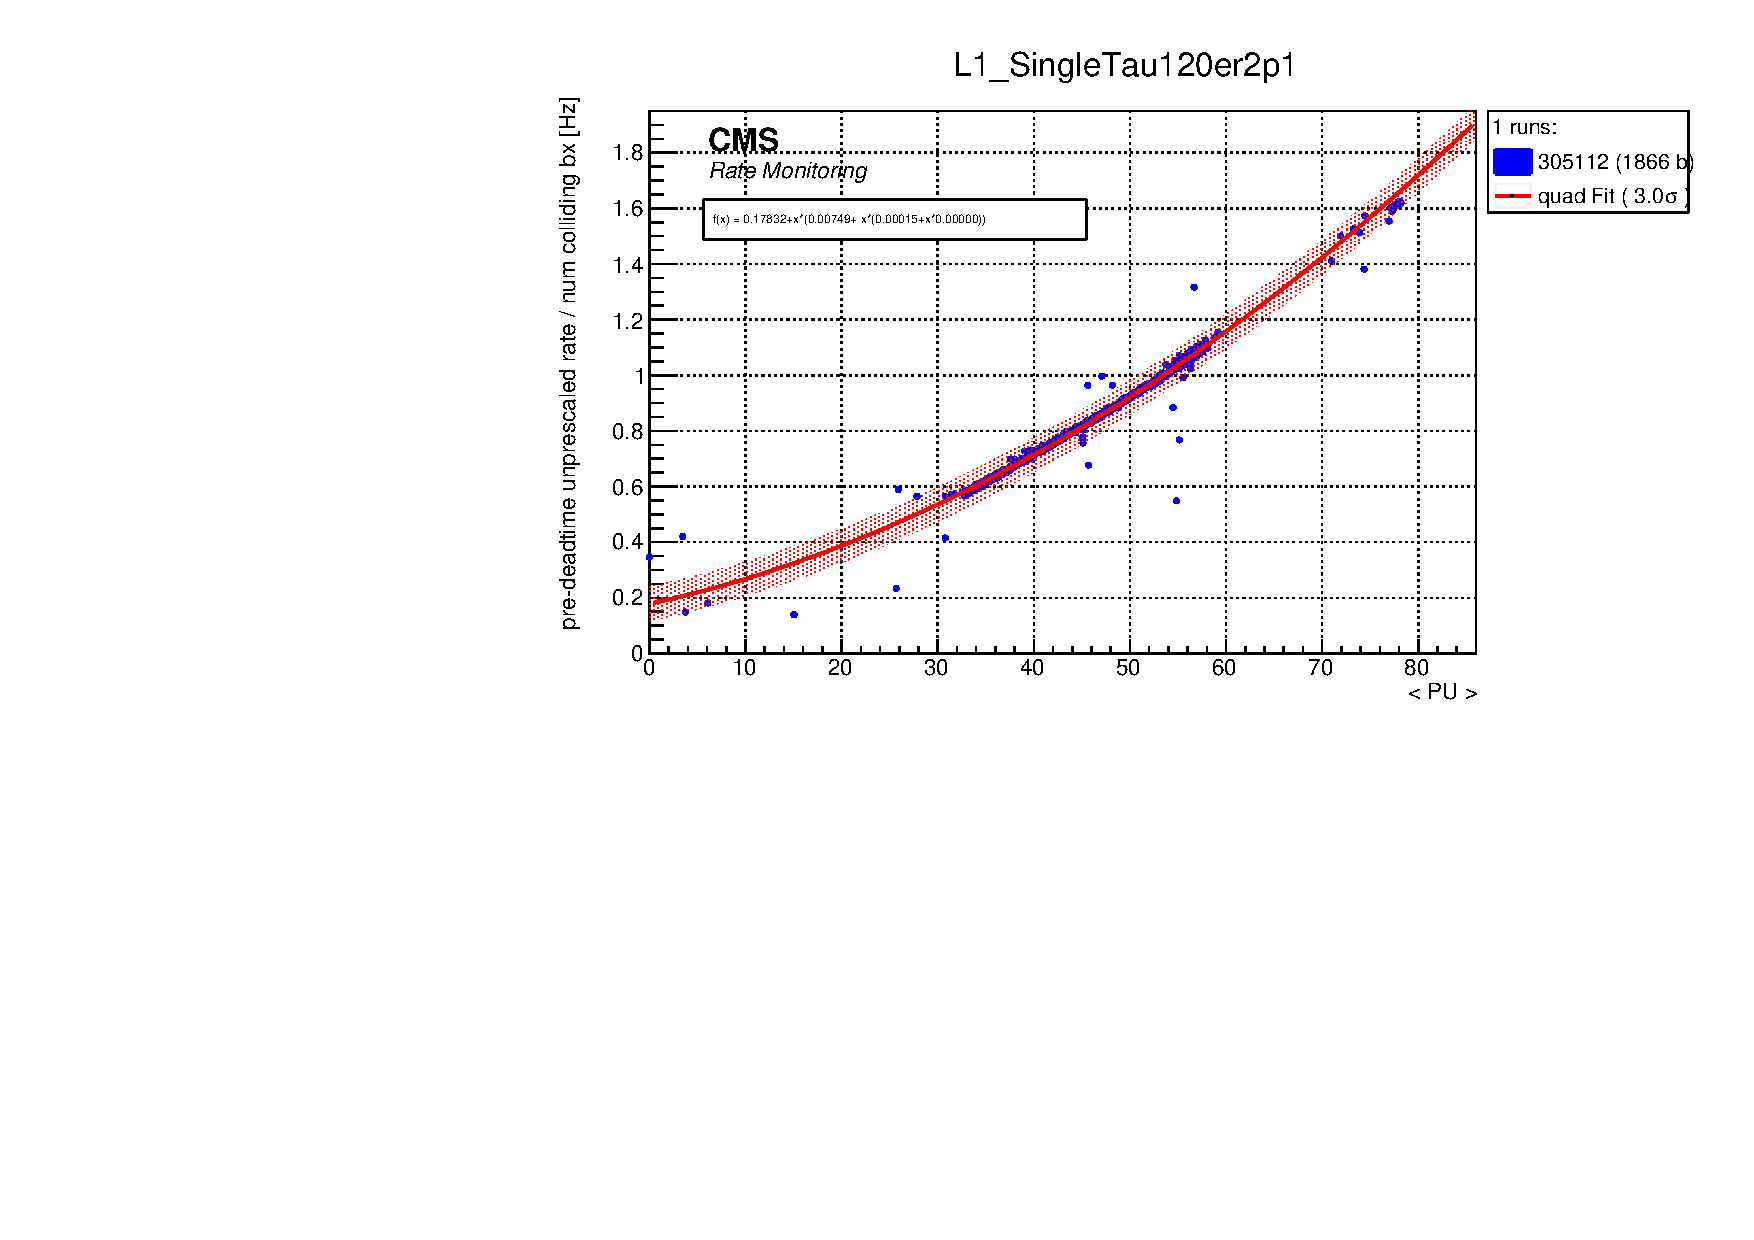
\includegraphics[width=0.6\paperwidth]{figures/RMT_305112_L1_SingleTau120er2p1.pdf}}
    \caption{L1 Trigger path plotted with a fitted function on run 305112}
    \label{fig:ratemon_l1}
\end{figure}

\begin{figure}
    \centerline{
        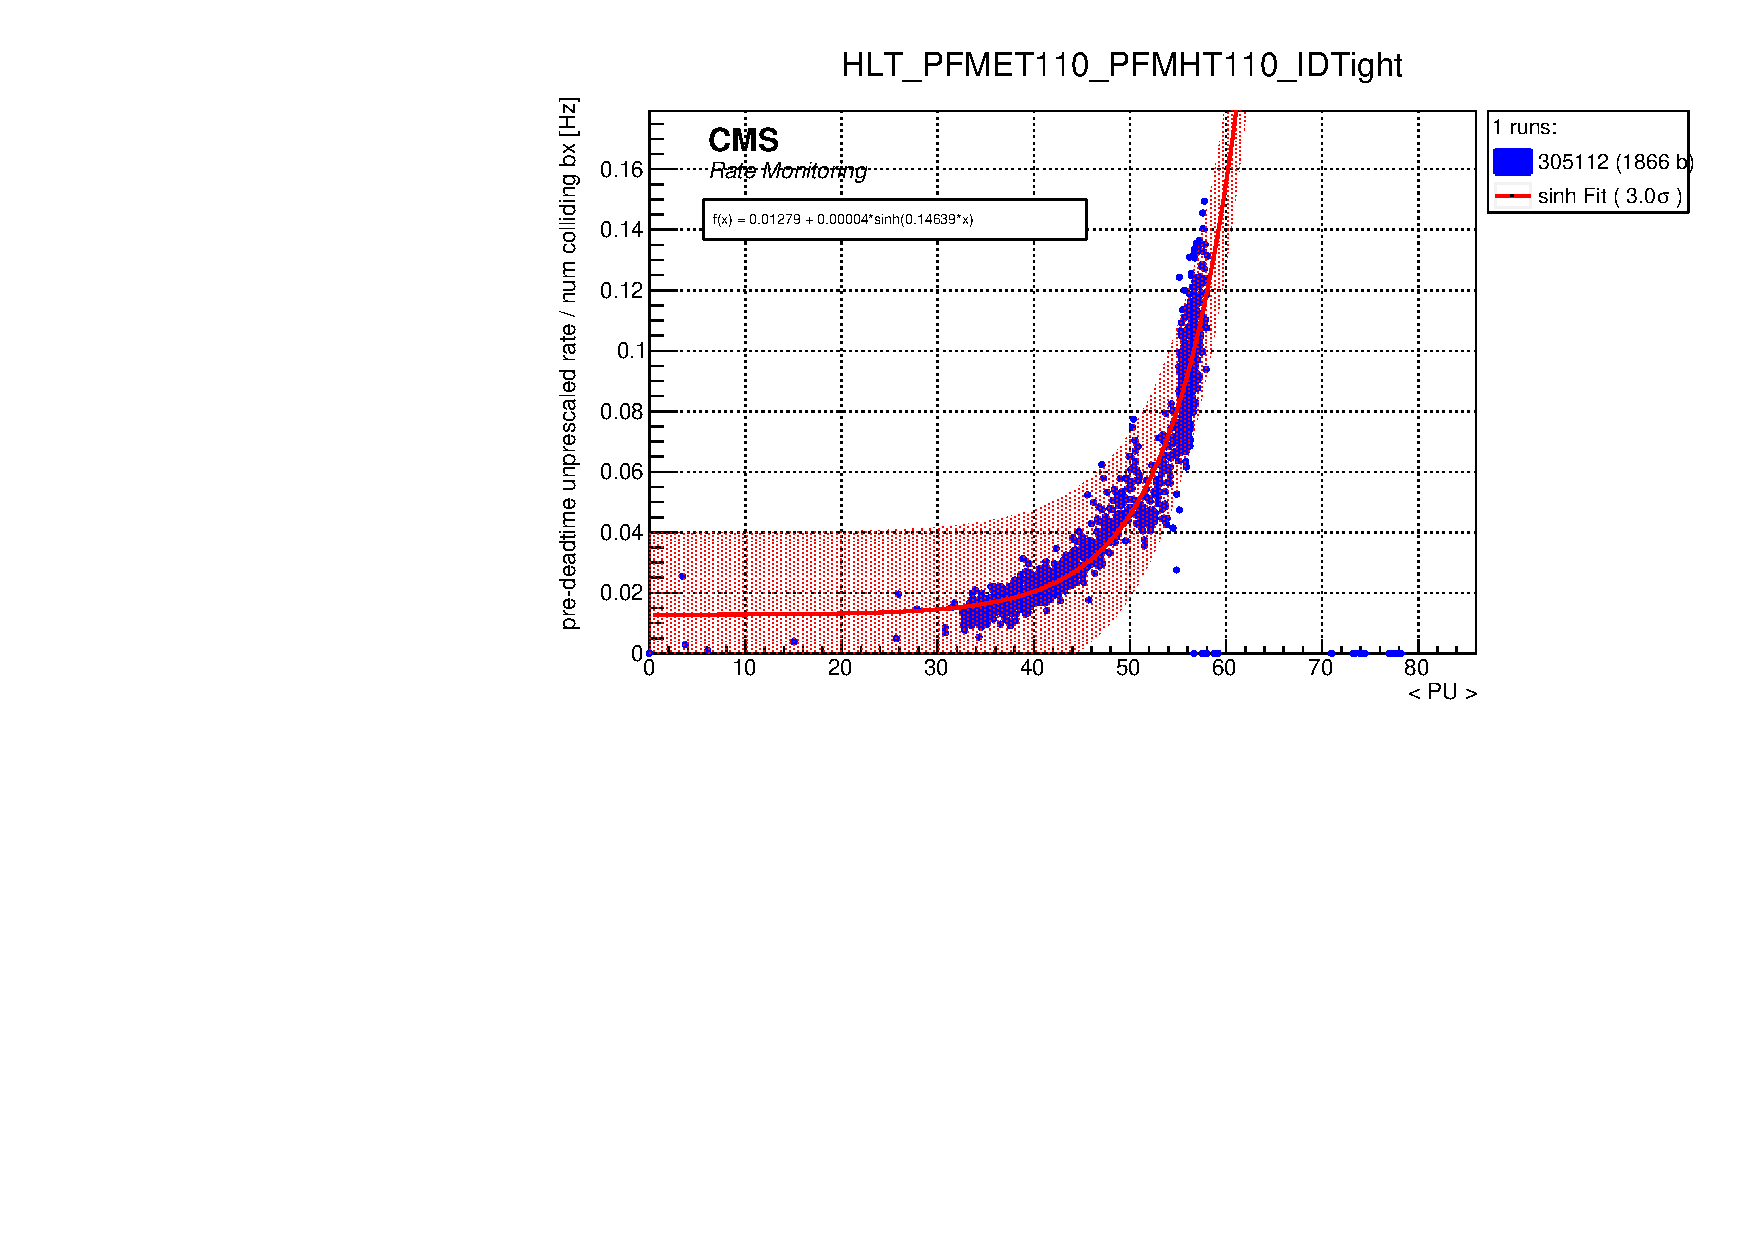
\includegraphics[width=0.6\paperwidth]{figures/RMT_305112_HLT_PFMET110_PFMHT110_IDTight.pdf}}
    \caption{HLT Trigger path plotted with a fitted function on run 305112}
    \label{fig:ratemon_hlt}
\end{figure}

These systems are continuosly monitored and their performance thoroughly evaluated. A survey of conferences, papers and technical reports on the tuning and performance evalution of the L1 Trigger is available in \cite{L1TriggerDPGResultsCMSPublicTWiki-2020-10-16}.

\section{Rate Monitoring software}

\subsection{Online Monitoring}

The High Level Trigger (HLT) rate monitoring tool is a python script that reports the rates of a selected list of triggers, primary datasets, and streams. It is run in the CMS control room and gives valuable real-time feedback of trigger rates to the shift crew: it updates every minute and averages the rates recorded in the last 3 lumisections, and, if possible, compares them to the predicted rate. Predictions are based on functions previously fitted on the same Trigger (\textit{fit functions}).

A list of \~{} 20 triggers is used for real-time online monitoring at point 5. This list is selected such that all CMS subdetectors are monitored and all physics objects are represented.

If a trigger path deviates by a specified amount from the prediction, or exceeds a fixed rate, the corresponding line is highlighted in a yellow colour. The scripts also displays other information that could be useful for the shifter, such as the run number and last lumisections, the LHC status, HLT key, deadtime, instantaneous luminosity and index of the prescale column in use.

When trigger rate exceeds the error band on the fit for a significant period of time (6 minutes, configurable), audible alarms are activated in the control room. Email warnings are sent to on-call experts.

\begin{figure}
    \centerline{
        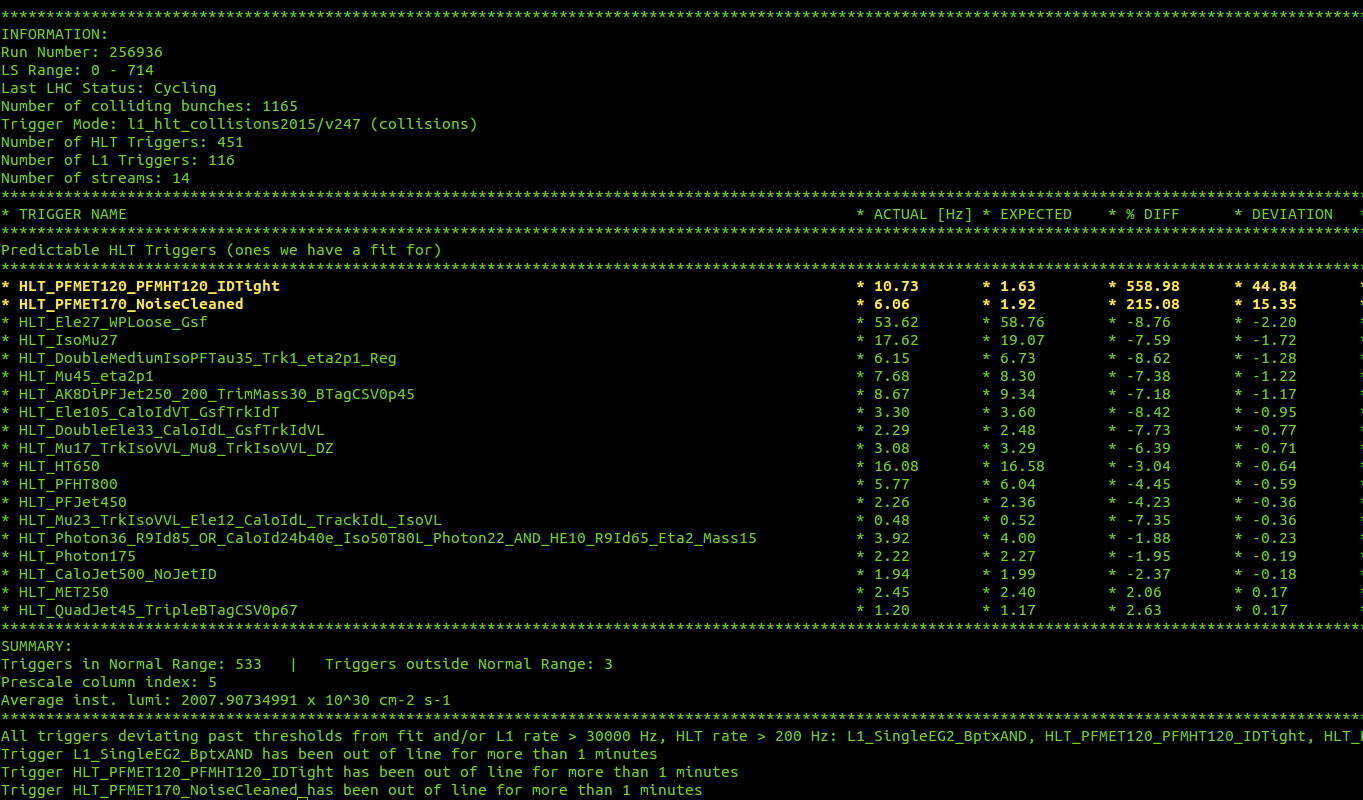
\includegraphics[width=0.8\paperwidth]{figures/ratemon_warnings}}
    \caption{Example execution of the Rate Monitoring Tool showing warnings: two triggers have values consistently deviating from the predictions. \cite{ratemon-twiki}}
    \label{fig:ratemon_warnings}
\end{figure}

\subsection{Plotting}

Another part of the software offers plotting features, exposed with the \mcode{plotTriggerRates} command line tool: it is used for observing how trigger rates vary over a range of beam and detector conditions, in particular how the rates of individual triggers scale with event pile-up.

Trigger Rates can be measured before of after the \textit{prescaling} and they can be adjusted or not for the \textit{deadtime}. They can also be plotted over the (time) progress of the run (LS, lumisections) instead of PU. Usually, they are represented in \textit{Rate vs. PileUp} plots, specifically "pre-deadtime unprescaled rate / num colliding bx [Hz]" over "PU" (Pile Up luminosity) units, generated by the RateMon tools.

In general, \textit{deadtime} refers to a time period during normal data taking when collisions are occurring but CMS is not ready to record the the data. This can occur for various reasons that are described in section 6.2.1 of \cite{Khachatryan_2017}. "pre-deadtime" rates are used in plots to allow for consistent comparison between different runs/fills; different runs and fills could have had different deadtimes, so correcting the rates for deadtime before fitting will allow the rates from different runs to be compared in a consistent way.

A \textit{prescale} is a way of scaling back the rate of L1 and HLT triggers. For example, if a certain trigger has a prescale of 5, then the data corresponding to the event the trigger fired on is only recorded once out of every five times that the trigger fired. So if the prescale is 1, the data will be recorded every time the trigger fires. A prescale of 0 means that no data will be recorded for the trigger in question: the trigger is essentially just turned off. Rates can be reported before this prescaling operation (\textit{unprescaled} or BP, before prescale) or after (\textit{prescaled}). Considering unprescaled rates enables comparisons across (different) pre scale columns.

\subsection{Alerting}

The trigger system regulates the massive data deluge coming from the observed collisions: its role is critical since any problem could result in a severe data loss. For this reason, the sub-detectors providing input to the trigger system and its output rates of accepted events need continuous "online" monitorng.

These rates affected by several issues: detector malfunctions, network or software problems, bad configurations. Examples of problems found by monitoring rates include: a failed  subdetector trigger hardware link, beam spot mis-alignment, luminometer calibration errors.

The current alerting strategy is based on the comparison between the observed per-node rate and its reference (predicted) value for the measured PU value. These references are derived from fitting previously collected data with analytical models.

\subsection{Fitting}

First, fits are made to the trigger rate in previous runs as a function of average pile-up (average number of collisions in an LHC bunch crossing). Runs to be fit are selected from a list of known good runs, and the fits are computed using ROOT. Before fitting, the raw trigger rate is first corrected for deadtime, prescales, and the the number of colliding bunches. Several fit functions are attempted, the final one is selected based on $\chi^2$ minimization \cite{Smith:2293136}.

Rates \textit{should} depend linearly on instantaneous luminosity, but some nonlinear behavior is observed, mainly due to the effects of pile-up: candidates for multiple object triggers may be found in independent collisions, and triggers (see \cite{Sirunyan:2721198} for accurate description of L1 triggers and \cite{Gori_2014} for HLT) that rely on measuring calorimeter deposits (such as jets and jet sums) increase in rate as the number of contributions from independent collisions increase.

Most triggers can be described with linear, quadratic, or exponential ($sinh$) functions.
 
\subsection{Offline use}

For a given list of runs and trigger paths, plots can be produced for an easy comparison by offline validators. A text summary reporting the deviating triggers is also produced.

\subsection{Overview}

A series of improvements and new features have been implemented on the Rate Monitoring tools, achieving the following goals:

\begin{enumerate}


        \item Upgraded the tools to run on a recent and supported version of Python (3.6) and updated the ROOT bindings.
        \item Moved the database connection configuration class to a separate and portable configuration file.
        \item Formally defined the environment and the dependencies needed to run the software.
        \item Prepared scripts to package the software with the RPM package format, to be compliant (and integrate) with the Control Room deployment procedures. Prepared a basic systemd service to include in the package, to allow running the software as a system service.
        \item Prepared a Continuos Integration and Deployment pipeline running on the CERN infrastructure.
        \item Upgraded the CI/CD pipeline to use the CMS Cactus \cite{DirkxCactus} auto DevOps tools.
        \item Upgraded the exporting feature of the tools, previously limited to shell output and small PNG image renders.
        \item Enabled the tools to export trigger rates data in ROOT binary files, allowing ROOT clients to read them.
        \item Enabled the tools to export trigger rates data also in a agnostic format, not tied to ROOT.
        \item Updated the documentation adding a way to consistently prepare any machine to run RateMon tools, without being tied to a particular machine cluster at CERN.
        \item Enabled any user to import the RateMon software as a Python module, adding some external-facing and transparent methods to get Trigger Rates as raw data or plots.
        \item Investigated a solution to integrate RateMon into the new CMS OMS, replacing the old WBM, now deprecated.
        \item Implemented an API exposing the exporting, processing and plotting functionalities of the RateMon software. This API is formally defined with an OpenAPI 3 Schema and an auto generated Swagger interface is available as documentation to users. This API can be plugged into the OMS stack to provide the old plots and many new features.
        \item Implemented a reactive web application in VueJS to demonstrate and showcase the API capabilities, plotting Trigger Rates (and their predicted values, based on the fits) in the browser with interactive and scalable plots (powered by JSROOT) instead of static image exports.
        \item Implemented a Trigger Selection interface on the UI, a feature requested by Trigger shifters and coordinators.
        \item Reported a series of bugs happening in the data querying and processing phase of the scripts, detailing test cases and scenarios triggering them, allowing future bug fixing work.
        \item Deployed the implemented stack in production and in the CMS Control Room. Set up a separate data storage solution to cache computed data, limiting the bottleneck effect of the CMS database on the API and offering faster responses.


\end{enumerate}

Each of these tasks will be detailed in this chapter, along with the rationale behind the choices made in the implementations.

A part from aiding the direct users of this tools, being able to consistently export rates from any trigger, run, fill, in any of the offered type of time series (Rate vs Pile Up, Rate vs Lumisection, ..) was also considered a prerequisite to do any kind of further data analysis study on this data.

\section{Infrastructure and tools}

We quickly introduce some tools and services we will be mentioning later, outlining their scopes in these operations.

\paragraph{SSH tunneling}

Some parts of the CERN infrastructure are accessible only when connected to the CERN Network. When this was not possible an SSH tunnel through LXPLUS was used to proxy the connection:

\begin{textcode}
$ ssh -D 1337 -q -N -f -C lxplus.cern.ch
\end{textcode}

A local SOCKS5 proxy is then available on the local machine. Any browser can be configured to use it, setting \mcode{localhost:1337} as proxy address. Tools like \mcode{tsocks} \cite{tsocksTransparentSOCKSProxyingLibrary-2020-10-07} or the more recently updated \mcode{proxychains-ng} \cite{proxychains-ng} can be used to run any command in the shell or launch any program transparently proxying the network connections trough the tunnel. E.g. to run Oracle SQL Developer and connect to the CMS OMDS database from outside CERN, \mcode{proxychains} can be configured in this way:

\begin{listing}[ht]
\begin{textcode}
# Strict - Each connection will be done via chained proxies
strict_chain
# Resolve DNS trough the proxy
proxy_dns
[ProxyList]
# localhost SSH tunnel
socks5  127.0.0.1 1337
\end{textcode}
\caption{/etc/proxychains.conf, proxychains configuration file}
\end{listing}

And then you are able to run

\begin{textcode}
$ proxychains ./sqldeveloper.sh
\end{textcode}

\paragraph{GitLab}

GitLab is a DevOps lifecycle tool, providing Git hosting, a wiki, issue-tracking, continuos integration and deployment features. There's a public instance running at GitLab.com, but the software is licensed with an "open-core" business model, so everyone can self-host the entire stack, provided they have the infrastructure.

GitLab business model is defined as "open core" (and not "open source"): core functionalities are offered as free and open source software, while additional commercial features, offered in the paid plans, are released under non-permissive license terms (source is still public).

In 2017, CERN chose GitLab as their code hosting solution and moved to a self-hosted GitLab instance. From now on, with "GitLab" we will refer to the CERN GitLab instance.

\paragraph{Docker containers}

Docker can package an application and its dependencies in a virtual container that can run on any Linux server. This enables the application to run in a variety of locations, mostly isolated from the host machine. Docker containers are defined by a single file, a Dockerfile.

\paragraph{Container Registry}

A stateless, highly scalable server side application that offers a storage and content delivery system, holding named Docker images, available in different tagged versions. With the Docker Container Registry integrated into GitLab, every GitLab project can have its own space to store its Docker images. Users interact with a registry by using docker push and pull commands.

\paragraph{EOS}

EOS \cite{Peters_2015} is an open source distributed low-latency disk storage system in production since 2011 at CERN. Having a highly-scalable hierarchical namespace, and with data access possible by the XROOT protocol, it was initially used for physics data storage. Today, EOS provides storage for both physics and user use cases.

\paragraph{CERNBox}

CERNBox \cite{Mascetti_2015} is the cloud data storage service available to all CERN users. It provides synchronisation and sharing clients for end users on all major platforms, including a web service. Core of the implementation is the XRootD framework providing a feature-rich remote access protocol. It is powered by the CERN EOS infrastructure as its storage backend.

\paragraph{WBM} The CMS Web Based Monitoring \cite{badgett2014web} is the old web portal that developed to present CMS monitoring and status information from many underlying heterogeneous sources, from real time messaging systems to relational database. In this being deprecated in favor of CMS OMS.

\paragraph{OMS} The CMS Online Monitoring System \cite{Andre2649402} is an upgrade and successor to the CMS Web-Based Monitoring (WBM) system, which is an essential tool for shift crew members, detector subsystem experts, operations coordinators, and those performing physics analyses. The CMS OMS is divided into aggregation and presentation layers. Communication between layers uses RESTful JSON:API compliant requests. The aggregation layer is responsible for collecting data from heterogeneous sources, storage of transformed and pre-calculated (aggregated) values and exposure of data via the RESTful API.The presentation layer displays detector information via a modern, user-friendly and customizable web interface.

\paragraph{ROOT} ROOT \cite{Brun:1997pa} is an open-source data analysis framework developed by CERN. It was originally designed for particle physics data analysis and contains several features specific to this field, but it is also used in other applications such as astronomy and data mining. It is used - through a Python interface, PyROOT \cite{PythoninterfacePyROOTROOT-2020-10-02} - in the RateMon software to process, normalise and plot trigger data.


\section{DevOps}

\subsection{Migration from GitHub}

The CMS Rate Monitoring git repository was hosted on GitHub. To enable Continues Integration and Continuos Deployment features, we migrated the repository to the CERN GitLab. The repository on GitHub is being kept as a mirror (as an additional git remote target) but the pipelines will be handled by GitLab.

\subsection{Folder Restructuring}

The folder has been restructured: the "misc" sub folder now contains the fits logs and the old scripts used with WBM (wbmRateReader). Everything was moved in "ratemon" sub folder, which will be the only one being packaged.

\subsection{Systemd service}

We prepared and included a systemd service file (\mcode{systemd/ratemon.service}), allowing the \mcode{ShiftMonitorTool} to be installed and used as a systemd service: running the \mcode{systemctl enable --now ratemon} command starts RateMon's ShiftMonitorTool "headlessly" and sets it to run at boot. Logs (previously shown on the shell running the script) can be viewed with \mcode{sudo journalctl -fu ratemon}. Trigger shifters are in the "systemd-journal" group and get access to this command without needing sudo or root permissions.


\subsection{Packaging}

The packaging phase is defined in the Makefile. We use \mcode{fpm} \cite{fpm-packager} to package the software in a RPM file with the given metadata and contents \cite{Packaging1MergeRequestsCMSTSGFOGratemonGitLab-2020-10-07}. Basically, the ratemon script folder is copied into \mcode{/opt/} \cite{FilesystemHierarchyStandard-2015-05-20} and the systemd service file goes into \mcode{/usr/lib/systemd/system}.

\begin{listing}[ht]
\begin{yamlcode}

RPM_NAME = ratemon-${VERSION}.${ARCH}.${BRANCH}.${HASH}.rpm

.PHONY: rpm
rpm: build ${RPM_NAME}
${RPM_NAME}:
  # Clean up the rpmroot directory
  rm -rf rpmroot
  # Create /opt
  mkdir -p rpmroot/opt
  # Systemd unit folder
  mkdir -p rpmroot/usr/lib/systemd/system
  # Copy the systemd unit file
  cp systemd/* rpmroot/usr/lib/systemd/system
  # Copy the ratemon folder
  cp -r ratemon rpmroot/opt

  # Launch fpm to package the prepared folder 
  fpm \
  -p ${RPM_NAME} \
  -n ratemon \
  -s dir \
  -t rpm \
  -v ${VERSION} \
  -a ${ARCH} \
  -d python3 -d root -d python36-root \
  --iteration ${RELEASE} \
  --description "Rate monitoring tools for HLT and L1" \
  --url "https://gitlab.cern.ch/cms-tsg-fog/ratemon" \
  --vendor "CERN" \
  rpmroot/=/
  mkdir -p rpms
  mv *.rpm rpms
\end{yamlcode}
\caption{Makefile "rpm" target launching the fpm tool to handle the packaging}
\end{listing}

Previously, the RateMon tools had to be installed checking out the code from the git repository, running a preparatory script, configuring the database connection and then running the script. Now, the system package manager can just install the packaged software:

\begin{textcode}
P5 $ yum install ratemon_0.1.rpm
\end{textcode}

RPM packages can be obtained on the repository "Releases" page, on public CERNBox or Dropbox folders or automatically installed in Puppet-managed machines, depending on the environment and system administration policy.

\subsection{Builder Docker image}

Starting from the \mcode{cern/cc7-base} base Docker image we prepared a "Builder" container, defined in \mcode{builder.Dockerfile}. It provides an isolated and reproducible environment in which we can run the building, packaging and deployment steps of the DevOps pipeline.
After pushing it to the Container Registry, it's exposed as \mcode{gitlab-registry.cern.ch/CMS-TSG-FOG/ratemon/builder}.

\begin{listing}[ht]
\begin{yamlcode}
FROM cern/cc7-base

RUN yum install -y ruby-devel gcc make rpm-build rubygems
RUN gem install --no-ri --no-rdoc fpm

CMD fpm
\end{yamlcode}
\caption{Builder.dockerfile}
\end{listing}


\subsection{CI/CD Pipeline}

\mcode{.GitLab-ci.yml} describes the GitLab CI. The first phase (\mcode{build\_rpm}) tells the builder (described by \mcode{builder.dockerfile} and exposed on the GitLab registry) to run \mcode{make rpm} (described in \mcode{Makefile}) and flags the produced RPM package files as artifacts; In the second phase (deploy), those artifacts are pushed on a EOS folder (\mcode{\/eos/user/a/avwebd2/ratemon\_builds}) using the ci-web-deployer tool with the credentials of a CERN Service Account (\mcode{avwebd2}).


\begin{listing}[ht]
\begin{yamlcode}

# EOS_PATH can be defined here or, if it needs to be hidden, 
# as a secure variable of the project (Settings -> CI/CD -> Variables)
# Note that the deploy-eos script needs the EOS_ACCOUNT_USERNAME and 
# EOS_ACCOUNT_PASSWORD of a secondary CERN account having write access on the
# specified EOS folder. Those are set as project variables.

variables:
  EOS_PATH: "/eos/user/a/avwebd2/ratemon_builds"

stages:
  - rpm
  - deploy

build_rpm:
  stage: rpm
  image: gitlab-registry.cern.ch/avivace/ratemon/builder
  script:
    # deploy-eos copies the content of the 'public' folder inside the specified
    # eos share
    - mkdir public
    - make rpm
    - mv *.rpm public/
  artifacts:
    paths:
      - public
    # Make it vanish in 1 hour
    expire_in: 1 hour

# https://gitlab.cern.ch/ci-tools/ci-web-deployer
deploy-eos:
  stage: deploy
  image: gitlab-registry.cern.ch/ci-tools/ci-web-deployer:latest
  script:
    - deploy-eos

\end{yamlcode}
\caption{First iteration of the CI/CD setup}
\end{listing}

\subsection{CMS Cactus}

CMS Cactus auto devops \cite{DirkxCactus} is a collection of GitLab CI templates and images designed to ease development and maintenance of CI workflows for Cactus projects. It is built on the same foundations as GitLab AutoDevOps, but tailored for CERN and CMS infrastructure.

As an additional improvement, we moved the CI/CD and packaging pipeline from vanilla’s GitLab tools to CMS Cactus, now using (and customising) a template provided by this tool.


\begin{listing}[ht]
\begin{yamlcode}

# include all templates in https://gitlab.cern.ch/cms-cactus/ops/auto-devops/-/tree/0.0.7
include:
  - project: cms-cactus/ops/auto-devops
    ref: 0.0.7
    file: templates/all.yml

# Only run when a branch or git tag is defined
# this avoids accidents like
# - detached pipelines causing undefined behavior
# - triggering for merge requests, where the CI pretends your code is already on the master branch, 
#   and thus you unintentionally push your RPMs to your production yum repo prematurely
workflow:
  rules:
  - if: $CI_COMMIT_TAG     
  - if: $CI_COMMIT_BRANCH

stages:
- setup
- build
- publish
- deploy

builder image:
  extends: .auto_devops_docker_builder_autotag_onchange
  stage: setup
  variables:
    DOCKERFILE: builder.Dockerfile
    CONTEXT_FOLDER: .gitlab/ci
    NAME: builder

make:
  image: $CI_REGISTRY_IMAGE/builder:$CI_COMMIT_REF_NAME-latest
  stage: build
  script:
  - make
  artifacts:
    paths:
    - "/rpms"

docker:
  extends: .auto_devops_docker_builder_autotag
  stage: publish
  variables:
    BUILD_ARG_CI_COMMIT_REF_NAME: $CI_COMMIT_REF_NAME

\end{yamlcode}
\caption{Setting up CI/CD by extending CMS Cactus templates}
\end{listing}


\section{Configuration}

A connection to the CMS OMDS database is required to run the software. Previously, the credentials needed to establish such connections had to be filled directly inside a python file imported by the application entry point.

The configuration file was moved to a YAML file, loaded using the \mcode{safe\_load} method offered by the PyYAML package \cite{pyyaml-2020-06-18}:

\mcode{safe\_load(stream)} parses the given stream and returns a Python object constructed from for the first document in the stream. If there are no documents in the stream, it returns \mcode{None}. \mcode{safe\_load} recognizes only standard YAML tags and cannot construct an arbitrary Python object.

Since we require just a couple of variables, this fits perfectly our use case, providing also a preliminary validation on the integrity of the file. The emitted Python object describing the configuration is then passed to the database connection class.

The \mcode{ShiftMonitorTool} and \mcode{plotTriggerRates} scripts now require an \mcode{--dbConfigFile} option, specifying the YAML configuration file containing the database connection parameters.

The documentation and the twiki page have been updated to reflect these changes. Scripts now need to be called in this way:

\begin{textcode}
$ python plotTriggerRates.py --dbConfigFile=dbConfig.yaml --useFills --createFit --bestFit --triggerList=TriggerLists/monitorlistCOLLISIONS.list 6303
\end{textcode}

\begin{listing}[ht]
\begin{yamlcode}
dsn_info:
    online: <value>
    offline: <value>

hlt_connect:
    user: <user>
    passwd: <passwd>

trg_connect:
    user: <user>
    passwd: <passwd>
\end{yamlcode}
\caption{dbConfig.yaml, the new required configuration file to run RateMon}
\end{listing}

\section{Exporting data}

The plots used to be rendered in small PNG images, with the resolution of 900$\times$600 pixels in a 8 bit color space. These images were then stored and served in the old Rate Monitoring page on WBM. No interactivity, navigation or filtering was possible, the only plots available were the Rate vs PU ones and the information about the fitted functions was not directly exposed.

\paragraph{Raw JSON}

The \mcode{plotTriggerRates} class was modified \cite{RootexporttoggleJSONexportfunction6MergeRequestsCMSTSGFOGratemonGitLab-2020-10-07} to be able to dump any Trigger Rate plot as a raw time series of plain numeric values in JSON files conform with a known \cite{avivacemasterthesisMyWIPmasterthesisinComputerScienceExperimentalAnomalyDetectiononCERNCMSTriggerRates-2020-10-16} schema. Additional meta data are included in the exported file too, such as the run number, the trigger key, the plotted variables and their units (e.g. Lumisection or PU as X, prescaled or unprescaled rate in Hz as Y), the coefficients and the form (e.g. linear or quadratic) of the fitted function.

This feature enables any plotting library to reconstruct the original plots and possibily draw the fit functions on the top of the time series.

The export can be toggled by passing the \mcode{--exportJSON} command line option.

\paragraph{ROOT files}

The possibility to export the plot canvas as a ROOT file has been added. This allows any ROOT instance to render the full plot natively.

This export functionality can be toggled by passing the \mcode{--exportRoot} command line option.

Rates for run (or for a fill) can now be exported:

\begin{itemize}
    \item As raw data, before any correction.
    \item With the corrections for deadtime applied.
    \item With the corrections for the prescale applied.
    \item With the corrections for colliding bunched applied.
    \item Over LS.
    \item Over the evolution of PU.
\end{itemize}

Some of these options can obviously be combined (e.g. \textit{pre-deadtime unprescaled}).

\section{Python3 upgrade}

Python 2.7 reached the end of life on the 1st January 2020. We made sure \cite{Python3migration4MergeRequestsCMSTSGFOGratemonGitLab-2020-10-07} that the tools could run under a recent and supported version of Python 3.

\section{From a CLI tool to a proper module}

The runstandalone method \cite{RestructuretheplotTriggerRatescripttobeusedasamodule7MergeRequestsCMSTSGFOGratemonGitLab-2020-10-07}


\begin{listing}[ht]
\begin{pythoncode}
# Exporting trigger rates importing the plotTriggerRates class
import plotTriggerRates as ptr
import yaml

# Read database configuration from file
with open("dbConfig.yaml", 'r') as stream:
    dbCfg = yaml.safe_load(stream)

# Specify which triggers we want
triggers = ["HLT_Ele40_WPTight_Gsf",
              "HLT_DoubleEle33_CaloIdL_MW"]

# Initialize the RateMon controller
controller = ptr.MonitorController()

# Get Trigger Rates from Fill 6303, creating fits
triggerrates = controller.runStandalone(
                         dbConfig=dbCfg,
                         triggerList=triggers,
                         useFills=True,
                         vsLS=False,
                         createFit=True,
                         bestFit=True,
                         data_lst=[6303])

# Print result
print(triggerrates)
\end{pythoncode}
\caption{Example usage of the RateMon module in a Python script}
\end{listing}

\section{API}

\cite{ExposefunctionalitieswithaRestfulAPI8MergeRequestsCMSTSGFOGratemonGitLab-2020-10-07}

\begin{figure}
    \centerline{
        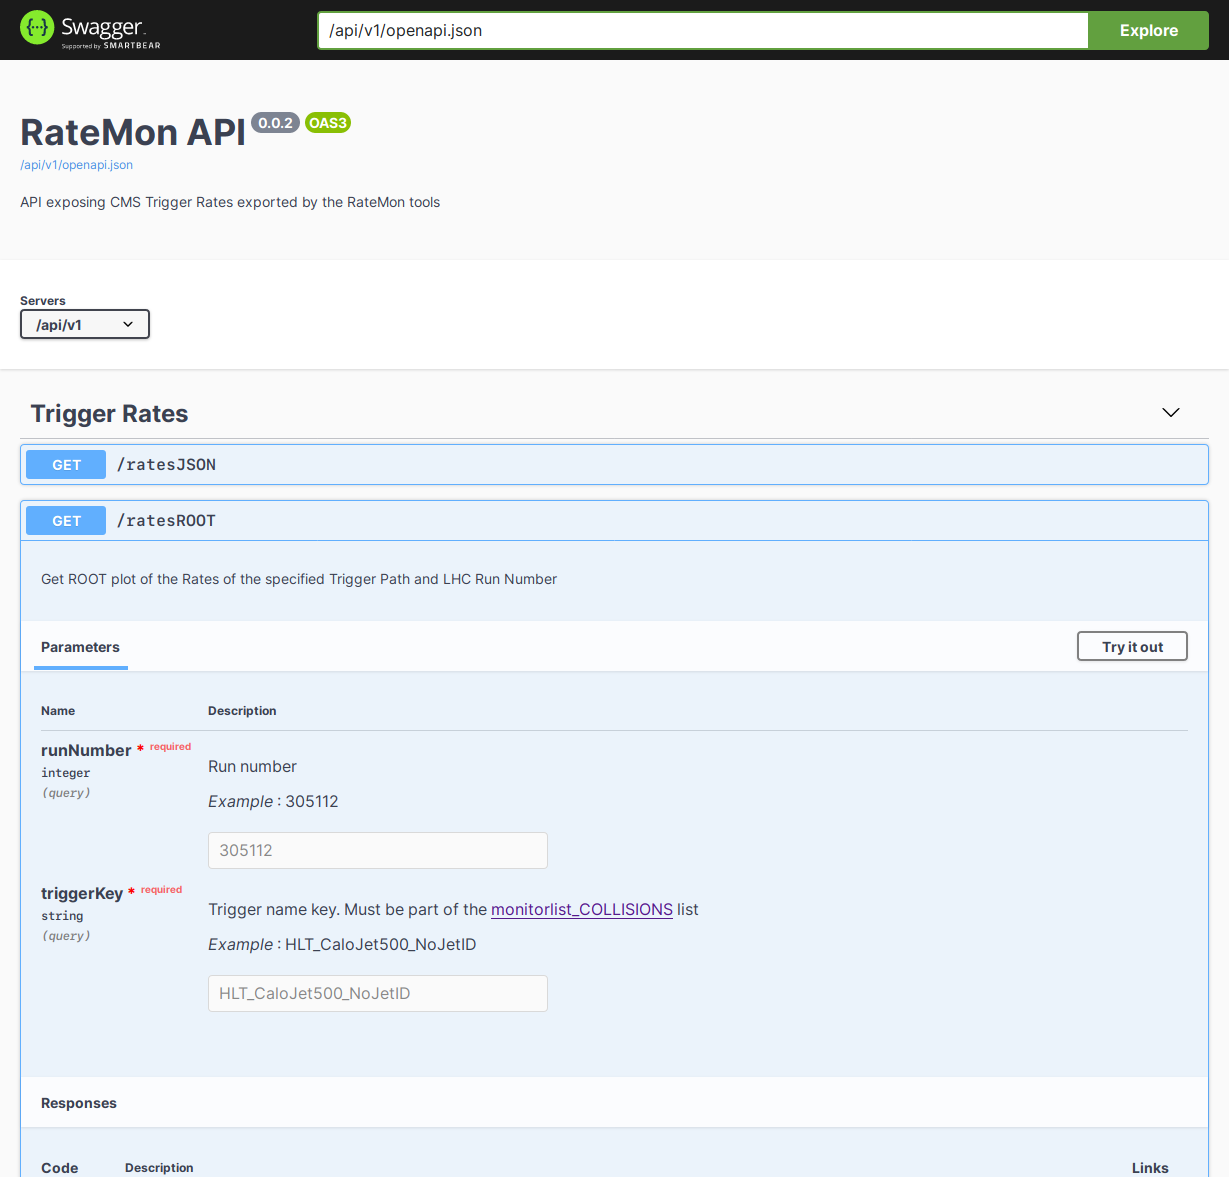
\includegraphics[width=0.8\paperwidth]{figures/swagger-ui}}
    \caption{Swagger UI}
    \label{fig:swagger-ui}
\end{figure}

\subsection{OpenAPI 3 Schema}

\begin{listing}[ht]
\begin{yamlcode}
openapi: "3.0.0"
info:
  version: 0.0.2
  title: RateMon API
  description: API exposing CMS Trigger Rates exported by the RateMon tools
servers:
  - url: http://ater.cern.ch/api/v1
paths:
  /ratesROOT:
    get:
      tags: [Trigger Rates]
      description: |
        Get ROOT plot of the Rates of the specified Trigger Path and LHC Run Number
      operationId: app.getRatesROOT
      parameters:
        - name: runNumber
          in: query
          description: "Run number"
          example: 305112
          required: true
          style: form
          schema:
            type: integer
        - name: triggerKey
          in: query
          description: "Trigger name key. Must be part of the [monitorlist_COLLISIONS](https://gitlab.cern.ch/cms-tsg-fog/ratemon/-/blob/api/ratemon/TriggerLists/monitorlist_COLLISIONS.list) list"
          example: HLT_CaloJet500_NoJetID
          required: true
          schema:
            type: string
      responses:
        '200':
          description: ROOT binary file of the computed plot
\end{yamlcode}
\caption{OpenAPI schema definition of the \texttt{/ratesROOT} API endpoint}
\end{listing}

Connexion, OpenAPI 3 schema, Swagger UI

\subsection{Implementation}

\begin{listing}[ht]
\begin{pythoncode}
def getRatesROOT(runNumber: int, triggerKey: str):
    saveDirectory = "/rtmdata/" + str(runNumber)
    rates = controller.runStandalone(
                         dbConfig=dbCfg,
                         exportRoot=True,
                         saveDirectory=saveDirectory,
                         makeTitle=False,
                         triggerList=[triggerKey],
                         createFit=True,
                         bestFit=True,
                         data_lst=[runNumber])

    return send_from_directory(saveDirectory,
                               triggerKey + '.ROOT',
                               as_attachment=True) # Keep the filename
\end{pythoncode}
\caption{Implementation of the \texttt{/ratesROOT} API endpoint}
\end{listing}

\subsection{Running}
\begin{textcode}
yum install libnsl

export LD_LIBRARY_PATH=/usr/lib/oracle/19.6/client64/lib:LD_LIBRARY_PATH

copy tnsnames.ora

wget https://download.oracle.com/otn_software/linux/instantclient/19600/oracle-instantclient19.6-basic-19.6.0.0.0-1.x86_64.rpm

yum install oracle-instantclient19.6-basic-19.6.0.0.0-1.x86_64.rpm
\end{textcode}

\section{Integration with OMS}

Highcharts, React, Panel

\section{Run Registry}

CMS Run Registry \cite{cms_collaboration_2019_3599323} is a in-development tool giving access to a lot of DQM datasets. TODO: describe bug reports, HTTPS auth problems and various contributions done upstream to this tool.

\cite{FixingtheBreakagefromtheAddTrustExternalCARootExpiration-2020-10-03} \cite{ErrorSSLCERTIFICATEVERIFYFAILEDIssue1CMSTrackerDPGcernrequests-2020-10-03} \cite{SSLerrorraisedbytheclientIssue1fabioespinosarunregistryapiclient-2020-10-03} \cite{WorkaroundskipSSLverificationbyavivacePullRequest2fabioespinosarunregistryapiclient-2020-10-03}

\section{API server deployment}

\subsection{Attaching a volume for caching}

To offer more disk space to the caching mechanism, a new volume has been created through the CERN Openstack infrastructure.

\begin{textcode}
lxplus $ # activate the correct OpenStack project
lxplus $ eval $(ai-rc 'Ratemon')
lxplus $ openstack volume create --description "Volume for RateMon API caching" --type standard --size 600 rtmcachevol
\end{textcode}

Size is measured in GB. The volume type "standard" is the default one, providing a reliable store which is tolerant to at least one disk failure without user impact or data loss. Maximum performance is 80 MB/s and 100 IO operations (both, read and write).

The command \mcode{openstack volume show} should now list the volume as available. We can attach it to the VM serving the API (\mcode{ater})

\begin{textcode}
lxplus $ openstack server add volume ater rtmcachevol
\end{textcode}

On the \mcode{ater} machine, \mcode{fdisk -l} will give the disks overview, listing the new volume. I noted the device ID (\mcode{/dev/vdb}) and then executed \mcode{fdisk /dev/vdb} to launch fdisk, the partition manager tool provided by the util-linux standard package.

\begin{textcode}
ater $ fdisk -l
...
Disk /dev/vdb: 600 GiB, 644245094400 bytes, 1258291200 sectors
Units: sectors of 1 * 512 = 512 bytes
Sector size (logical/physical): 512 bytes / 512 bytes
I/O size (minimum/optimal): 512 bytes / 512 bytes
\end{textcode}

In the fdisk shell, create a new partition (\mcode{n}), select is a primary (\mcode{p}) and denote it as the first (\mcode{1}). Set it to occupy all the available space accepting defaults. Select again the partition (\mcode{t}) and set the Linux partition type (\mcode{83}). (\mcode{p}) displays the partition setup we just defined. If that's okay, (\mcode{w}) commits the modifications and applies them.

\begin{textcode}
Device     Boot Start        End    Sectors  Size Id Type
/dev/vdb1        2048 1258291199 1258289152  600G 83 Linux
\end{textcode}

Back in the standard shell, use \mcode{mkfs.ext4 /dev/vdb} to format the partition using the EXT4 file system.

Note the UUID of our newly formatted partition:

\begin{textcode}
ater $ mkfs.ext4 /dev/vdb
mke2fs 1.45.4 (23-Sep-2019)
Creating filesystem with 157286400 4k blocks and 39321600 inodes
Filesystem UUID: f74a87c8-7ced-4414-bc62-e09d07be7845
\end{textcode}

Now that we know the UUID, we can mount the volume:

\begin{textcode}
ater $ mkdir /cache
ater $ mount /dev/disk/by-uuid/f74a87c8-7ced-4414-bc62-e09d07be7845 /cache
\end{textcode}

To make the mounting persistent, we add this entry to the \mcode{/etc/fstab} file:

\begin{textcode}
UUID=f74a87c8-7ced-4414-bc62-e09d07be7845   /cache  auto defaults,nofail    0 3
\end{textcode}

Here's the final situation, as described by \mcode{df -h}:

\begin{textcode}
ater $ df -h
Filesystem      Size  Used Avail Use% Mounted on
...
/dev/vda2        40G   33G  7.6G  82% /
/dev/vdb        590G   73M  560G   1% /cache
\end{textcode}

\subsection{NGINX as reverse proxy and cache server}


\begin{textcode}
sudo cat /var/log/audit/audit.log | grep nginx | grep denied
\end{textcode}


\begin{textcode}
$ setsebool -P httpd_can_network_connect 1
$ chown nginx:nginx /cache/
\end{textcode}


\begin{listing}[ht]
\begin{nginxcode}
# Set cache dir
proxy_cache_path /cache levels=1:2 keys_zone=one:50m max_size=500g inactive=200d;

# Set cache key to include identifying components
proxy_cache_key $scheme$proxy_host$request_uri;

# Add cache status to log
log_format cache '$remote_addr - $remote_user [$time_local] "$request" $status $body_bytes_sent "$http_referer" "$http_user_agent" cs=$upstream_cache_status';

server {
    server_name ater.cern.ch;
    add_header X-Cache-Status $upstream_cache_status;
    
    ## Access and error logs.
    access_log /var/log/nginx/api-proxy.access.log cache;
    error_log  /var/log/nginx/api-cache.error.log;  
    
    location / {
        proxy_set_header Host $host;
        proxy_set_header X-Real-IP $remote_addr;
            
        proxy_cache one;
        proxy_ignore_headers X-Accel-Expires Expires Cache-Control;
        proxy_cache_valid 200 302 200d;
        proxy_cache_valid 404 15m;
        proxy_pass http://localhost:8085;   
    
    }
    listen 80;
}
\end{nginxcode}
\caption{NGINX configuration for reverse proxying and caching}
\end{listing}

\section{A new User Interface}

VueJS \cite{Vuejs-2020-10-04}, Vuetify \cite{VuetifyAMaterialDesignFrameworkforVuejs-2020-10-04} ROOT, Plotly, Plotly -> JSROOT \cite{JavaScriptROOT-2020-05-07}

\begin{figure}
    \centerline{
        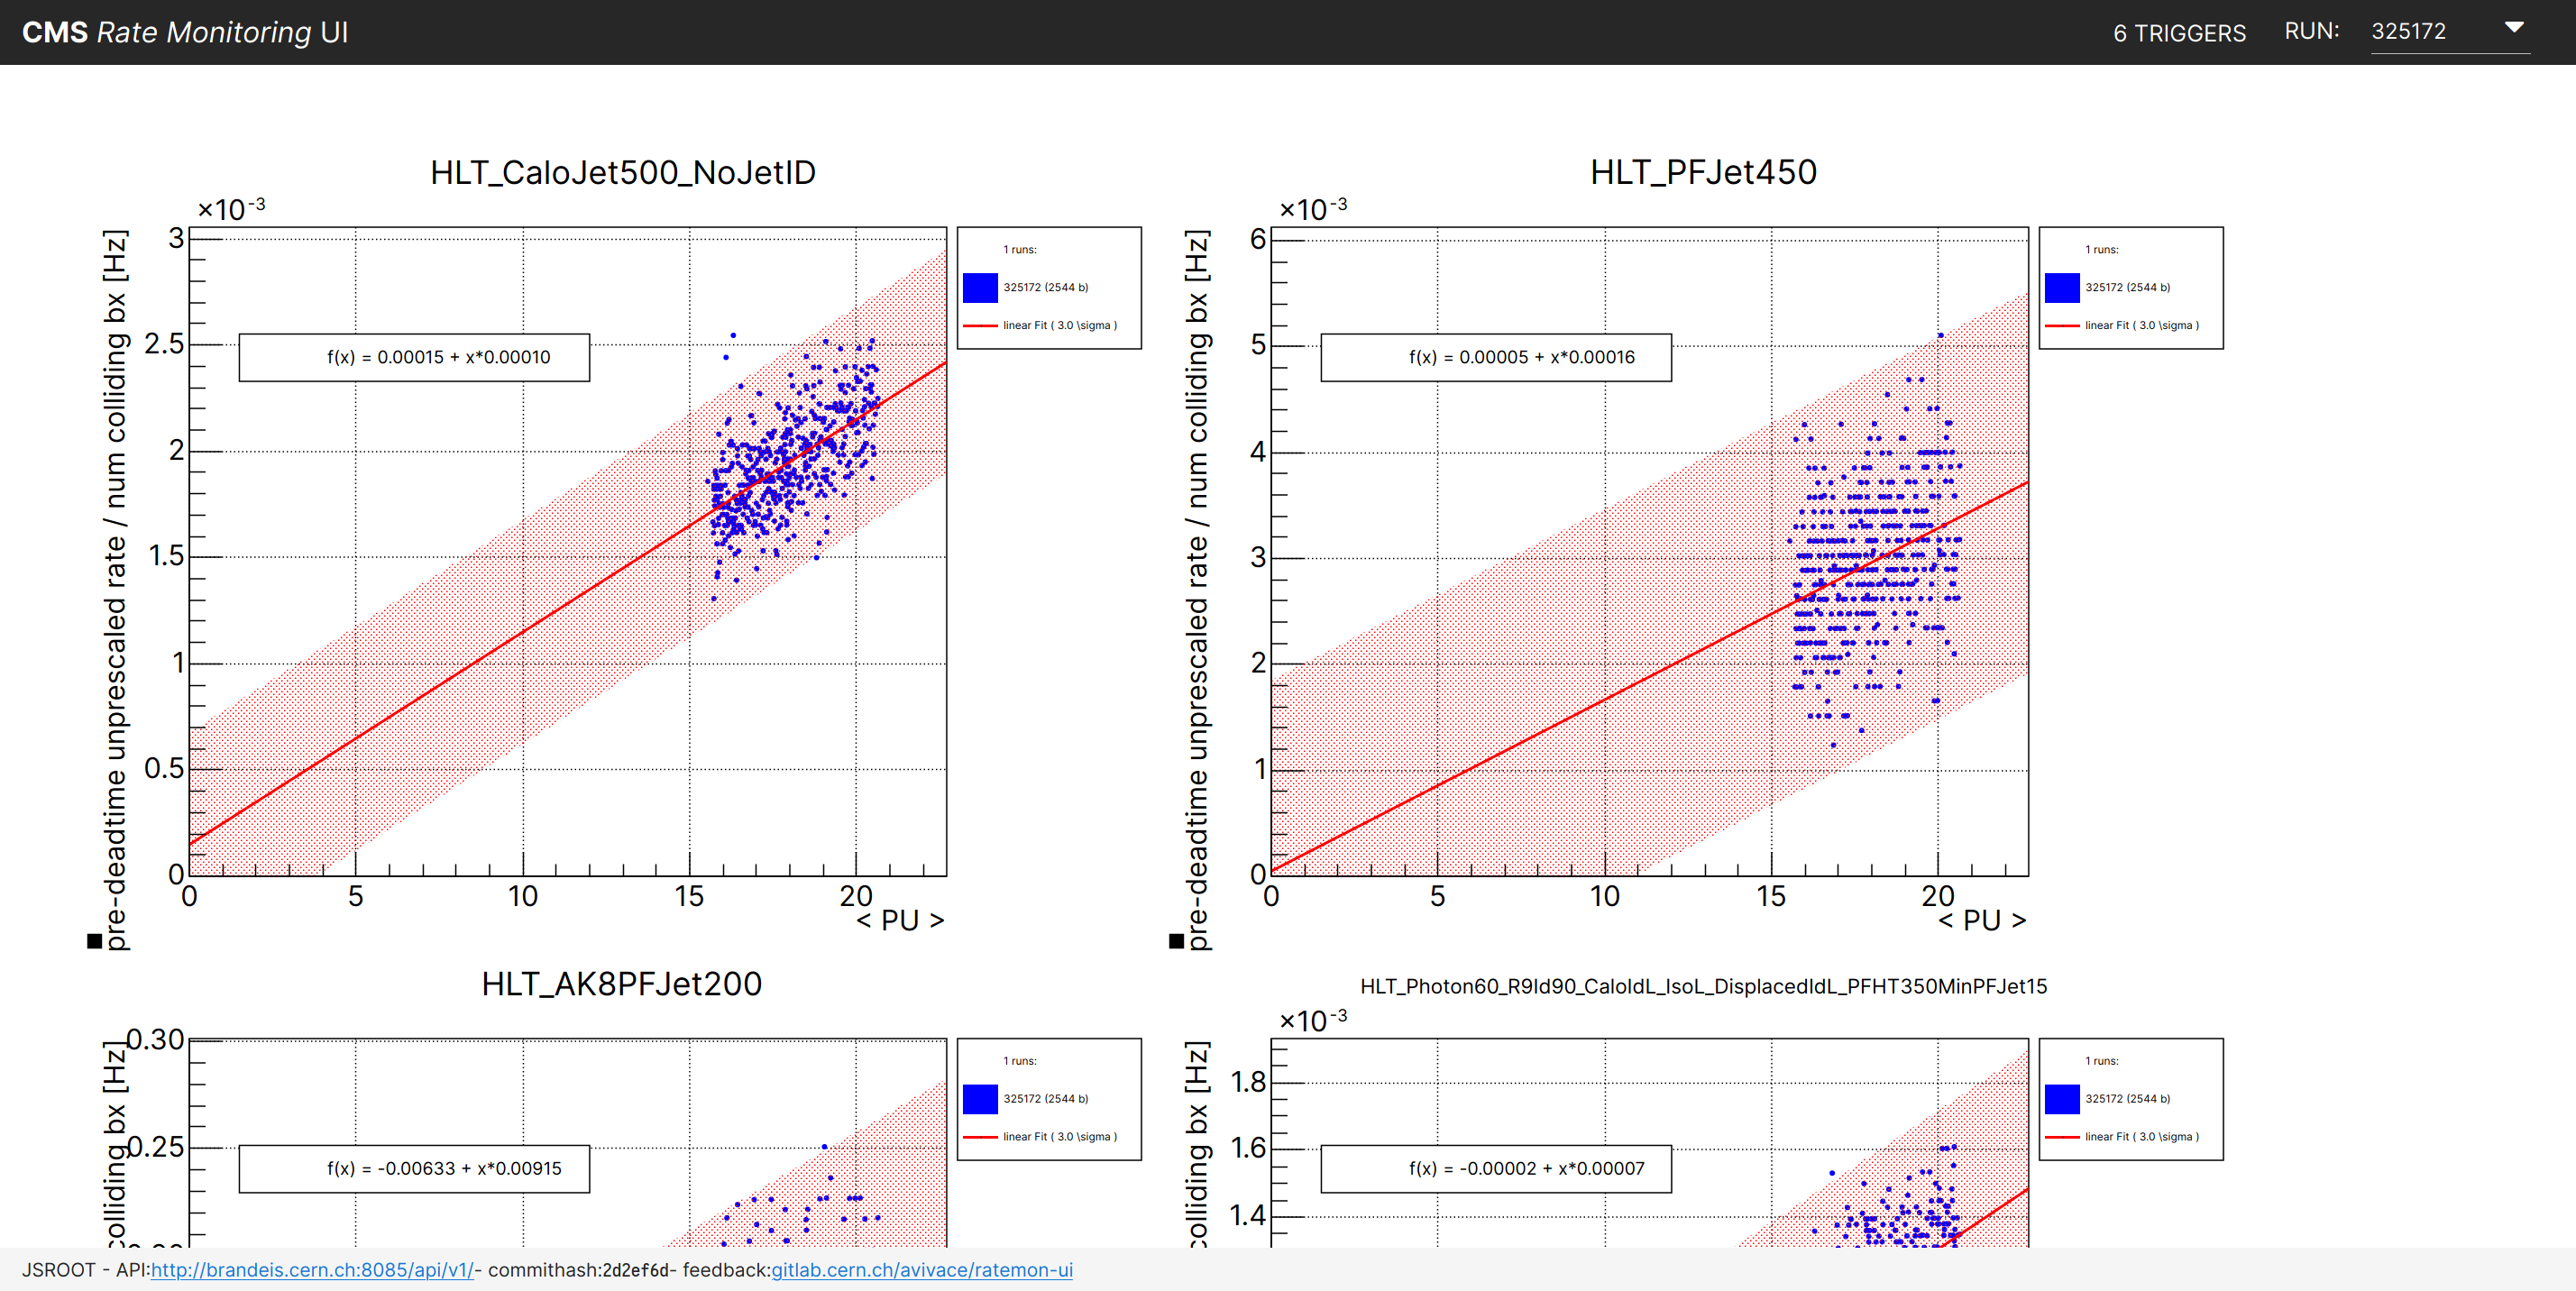
\includegraphics[width=0.9\paperwidth]{figures/ratemon-ui0.png}}
    \caption{Main RateMon UI application view, showing interactive trigger rate plots and relative fit functions}
    \label{fig:ratemon_ui0}
\end{figure}

\begin{figure}
    \centerline{
        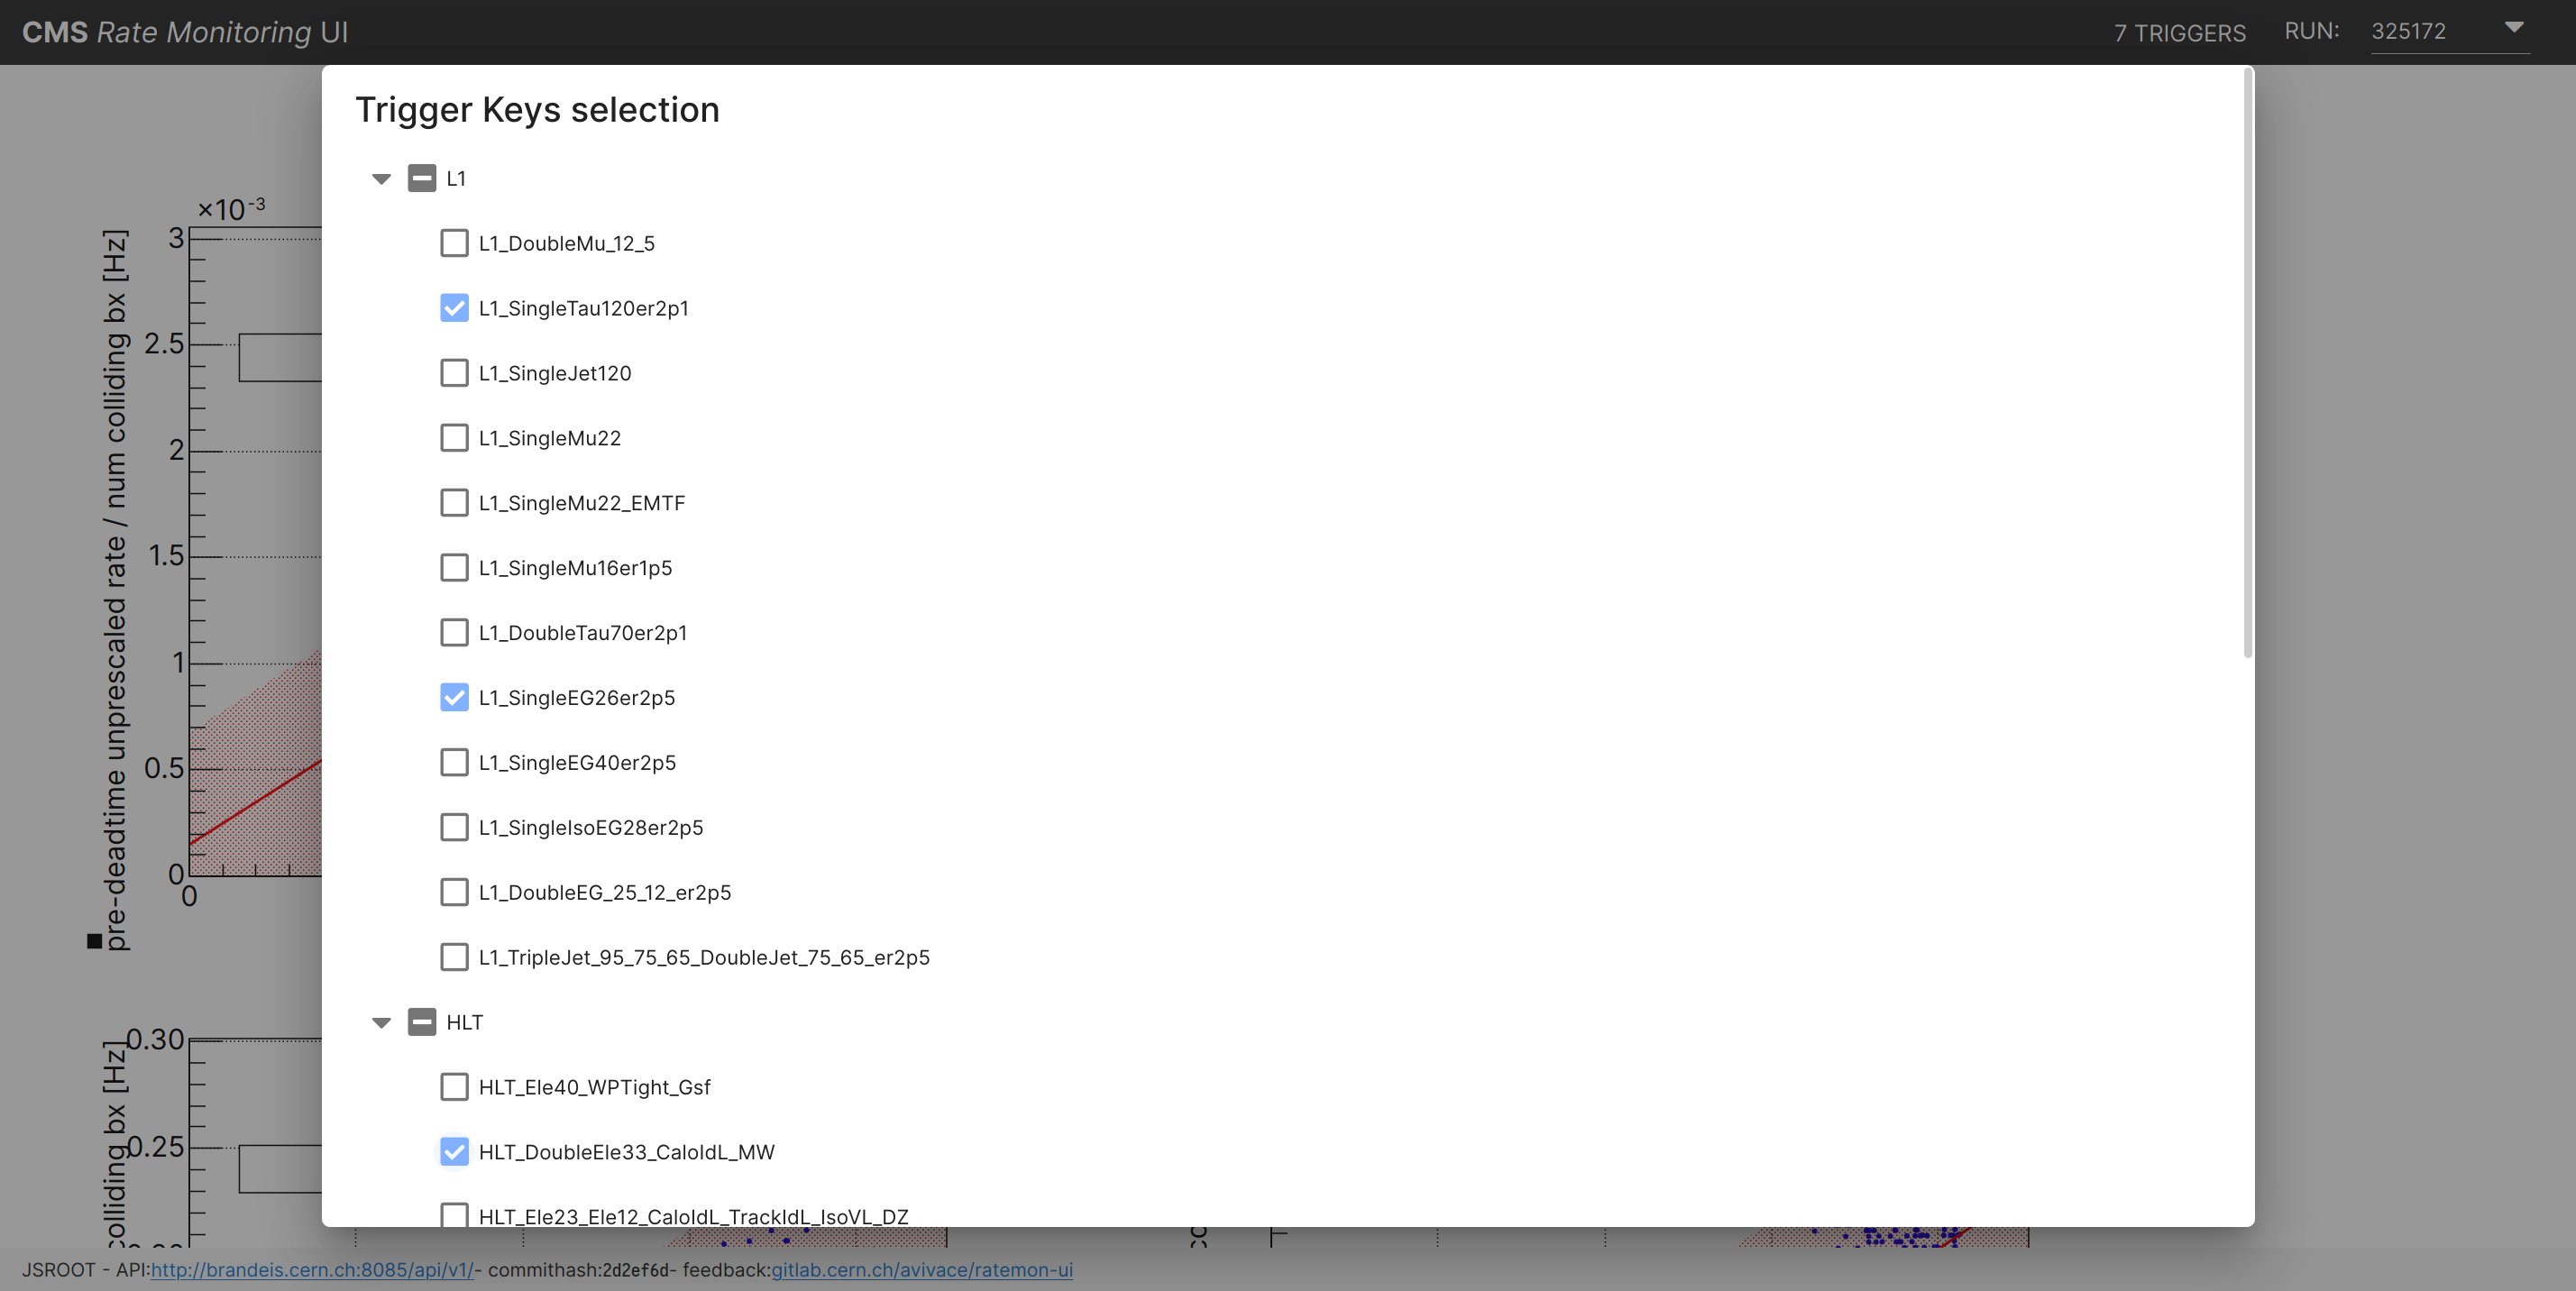
\includegraphics[width=0.9\paperwidth]{figures/ratemon-ui1.png}}
    \caption{Trigger selection in the RateMon UI}
    \label{fig:ratemon_ui0}
\end{figure}